%! TEX root = thesis.tex

\chapter{Software Architecture and Implementation}
\label{sec:implementation}

\section{Technology Stack}
\label{sec:tech-stack}

The Green Epoch application is implemented as a fully client-side single-page
application using SolidJS with TypeScript.  The entire simulation engine
and optimizer run in the browser; the server only serves static files.  This
architecture eliminates backend dependencies, reduces operational cost, and
makes the application accessible to anyone with a web browser.

\begin{itemize}
  \item \textbf{Frontend framework:} SolidJS 1.9 with reactive state
    management, compiled by Vite.
  \item \textbf{Styling:} Tailwind CSS 4 with dark and light mode support.
  \item \textbf{Charts:} Chart.js for time-series carbon intensity plots,
    Plotly for 3D scatter visualization of the optimization space.
  \item \textbf{Simulation:} Pure TypeScript domain logic, run inside Web
    Workers for non-blocking execution.
  \item \textbf{Testing:} Vitest with testing-library for component and
    unit tests.
  \item \textbf{CLI:} Commander.js-based command-line interface for headless
    simulation and optimization.
\end{itemize}

\section{Architecture Overview}
\label{sec:architecture}

The application follows a three-layer architecture that separates pure business
logic from execution and presentation:

\begin{description}
  \item[Domain layer:] Pure TypeScript modules with no UI or side-effect
    dependencies.  Contains the simulation step engine, physics constants,
    hysteresis policy, scoring functions, and the adaptive grid-search
    optimizer.  This layer is fully portable and is also used by the CLI.
  \item[Engine layer:] Web Worker wrappers that offload simulation,
    optimization, batch runs, and CO$_2$ data loading to background threads.
    Each worker communicates with the UI via message passing, posting progress
    updates and results asynchronously.
  \item[UI layer:] SolidJS page components implementing the four main views:
    scenarios overview, single-run simulation, batch run dashboard, and
    optimization page.  Reusable components include the CO$_2$ time-series
    chart, stats panels, scenario forms, and the 3D optimization plot.
\end{description}

Figure~\ref{fig:scenarios-overview} shows the scenarios overview page where users manage their simulation configurations.

\begin{figure}
  \centering
  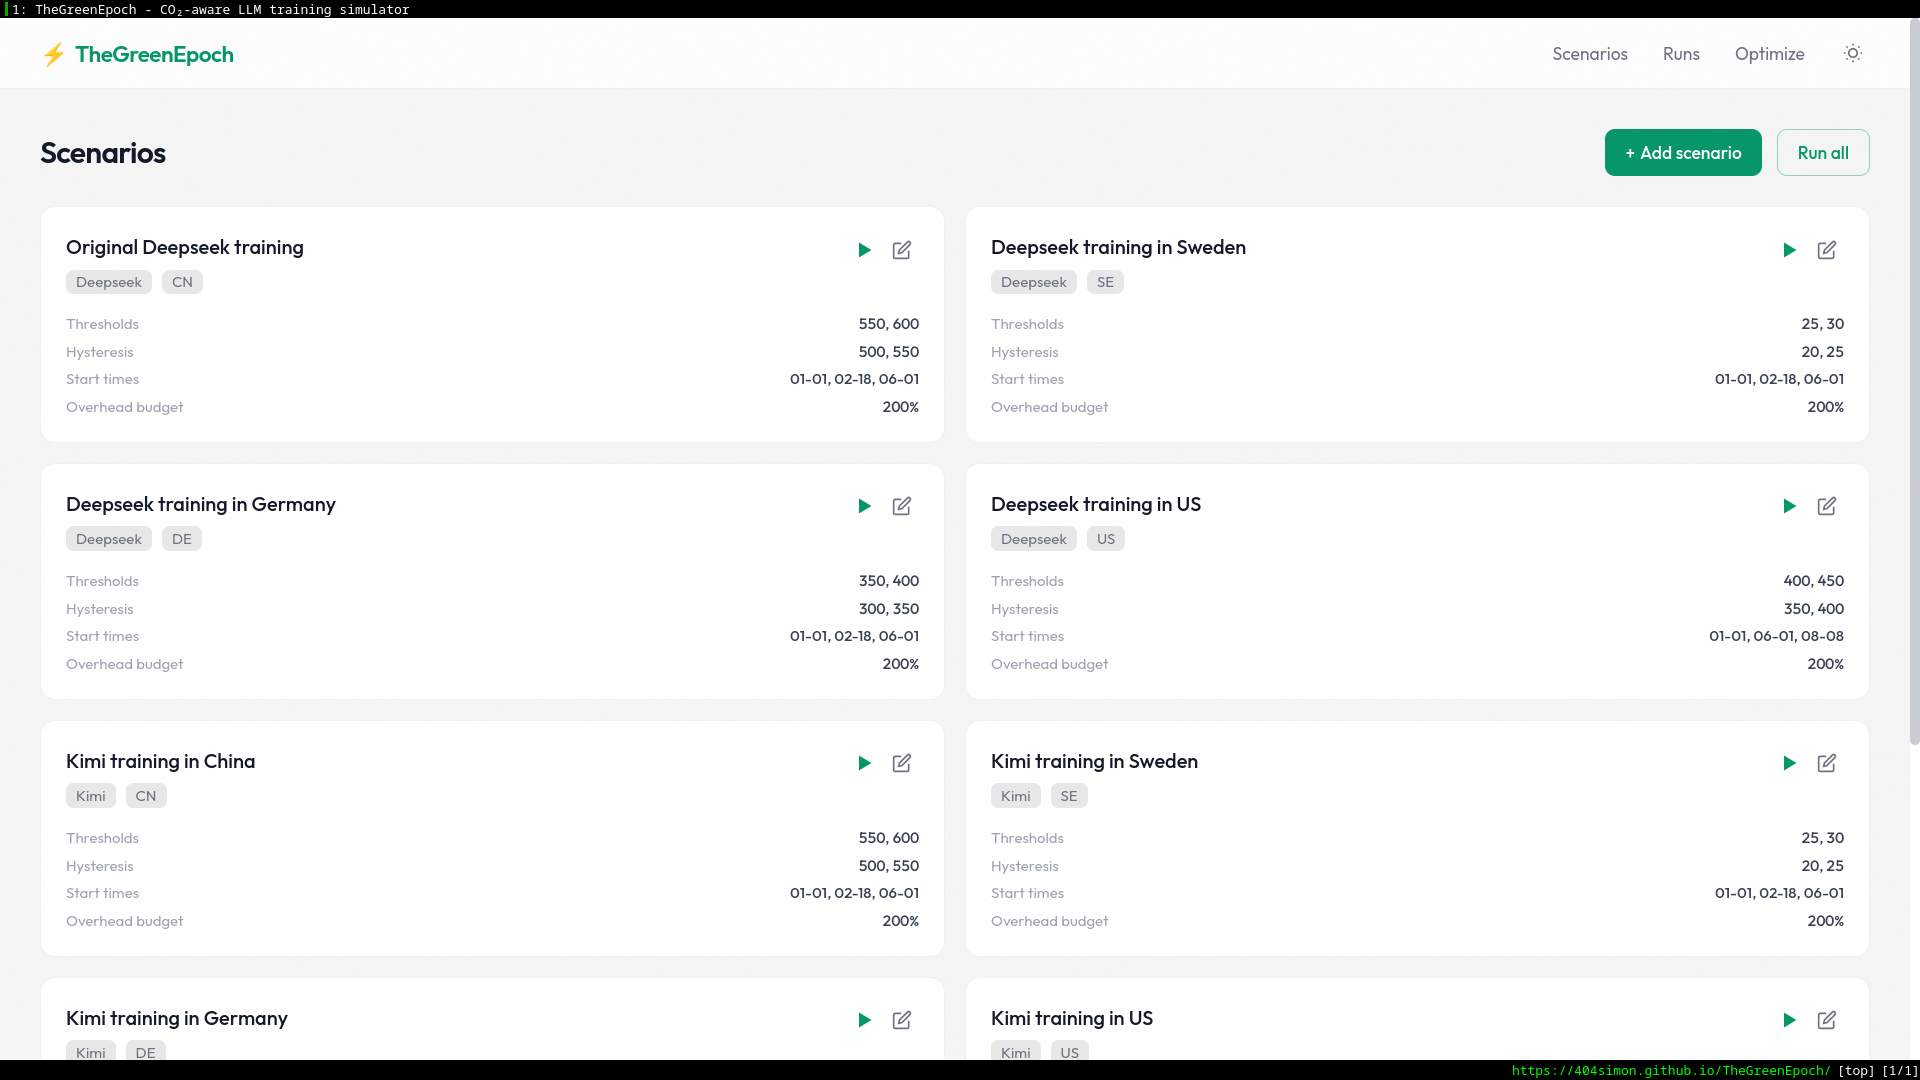
\includegraphics[width=\textwidth]{figures/screenshots/scenarios_overview_page}
  \caption{Scenarios overview page: users can view, create, edit, and launch
  simulation scenarios.}
  \label{fig:scenarios-overview}
\end{figure}

\section{Simulation Engine}
\label{sec:simulation-engine}

The simulation engine is the core of the domain layer.  It exposes a single
generator function \texttt{simulateStepwise()} that yields simulation state
at each timestep.  This design enables both real-time visualization (by
consuming the generator incrementally) and batch execution (by draining it to
completion).

Key design decisions include:
\begin{itemize}
  \item \textbf{Timestep alignment.} The CO$_2$ timeline is indexed by Unix
    timestamp.  The simulator advances through the timeline in 5-minute steps,
    querying the current intensity via binary search.
  \item \textbf{State machine.} The pause/resume logic is implemented as a
    deterministic finite state machine with four states: training, pausing
    (checkpoint save), paused, and resuming (checkpoint load).
  \item \textbf{Progress accounting.} Training progress increments only during
    the training state.  Baseline duration is computed from the training
    profile (tokens, GPU-hours, GPU count).  Wall-clock time accumulates
    across all states.
\end{itemize}

The interactive simulation view is shown in Figure~\ref{fig:single-run-top}, which displays the CO$_2$ intensity chart with threshold annotations and real-time KPIs. Figure~\ref{fig:single-run-bottom} presents the detailed comparison against the never-pause baseline below the chart area.

\begin{figure}
  \centering
  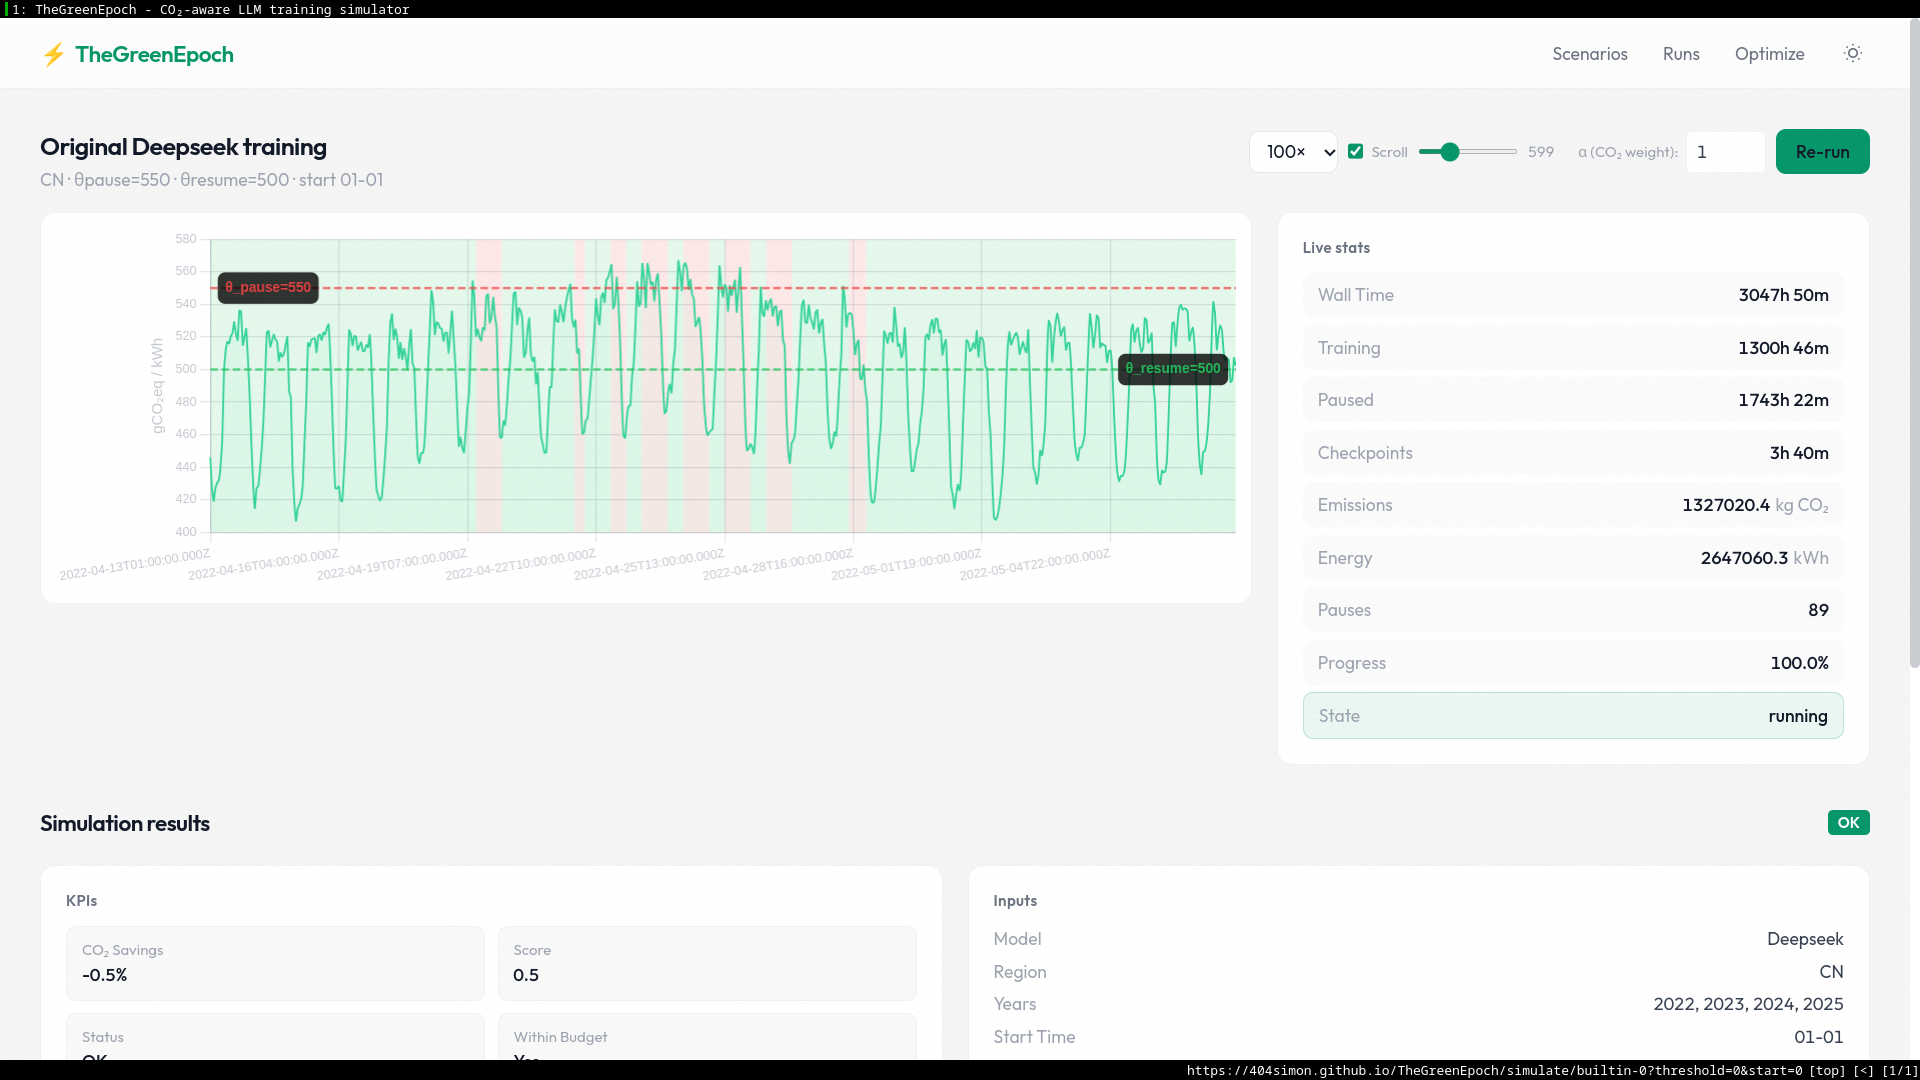
\includegraphics[width=\textwidth]{figures/screenshots/single_scenario_run_top_page}
  \caption{Single scenario run view: interactive simulation with CO$_2$
  intensity chart, pause/resume threshold annotations, and real-time
  statistics.}
  \label{fig:single-run-top}
\end{figure}

\begin{figure}
  \centering
  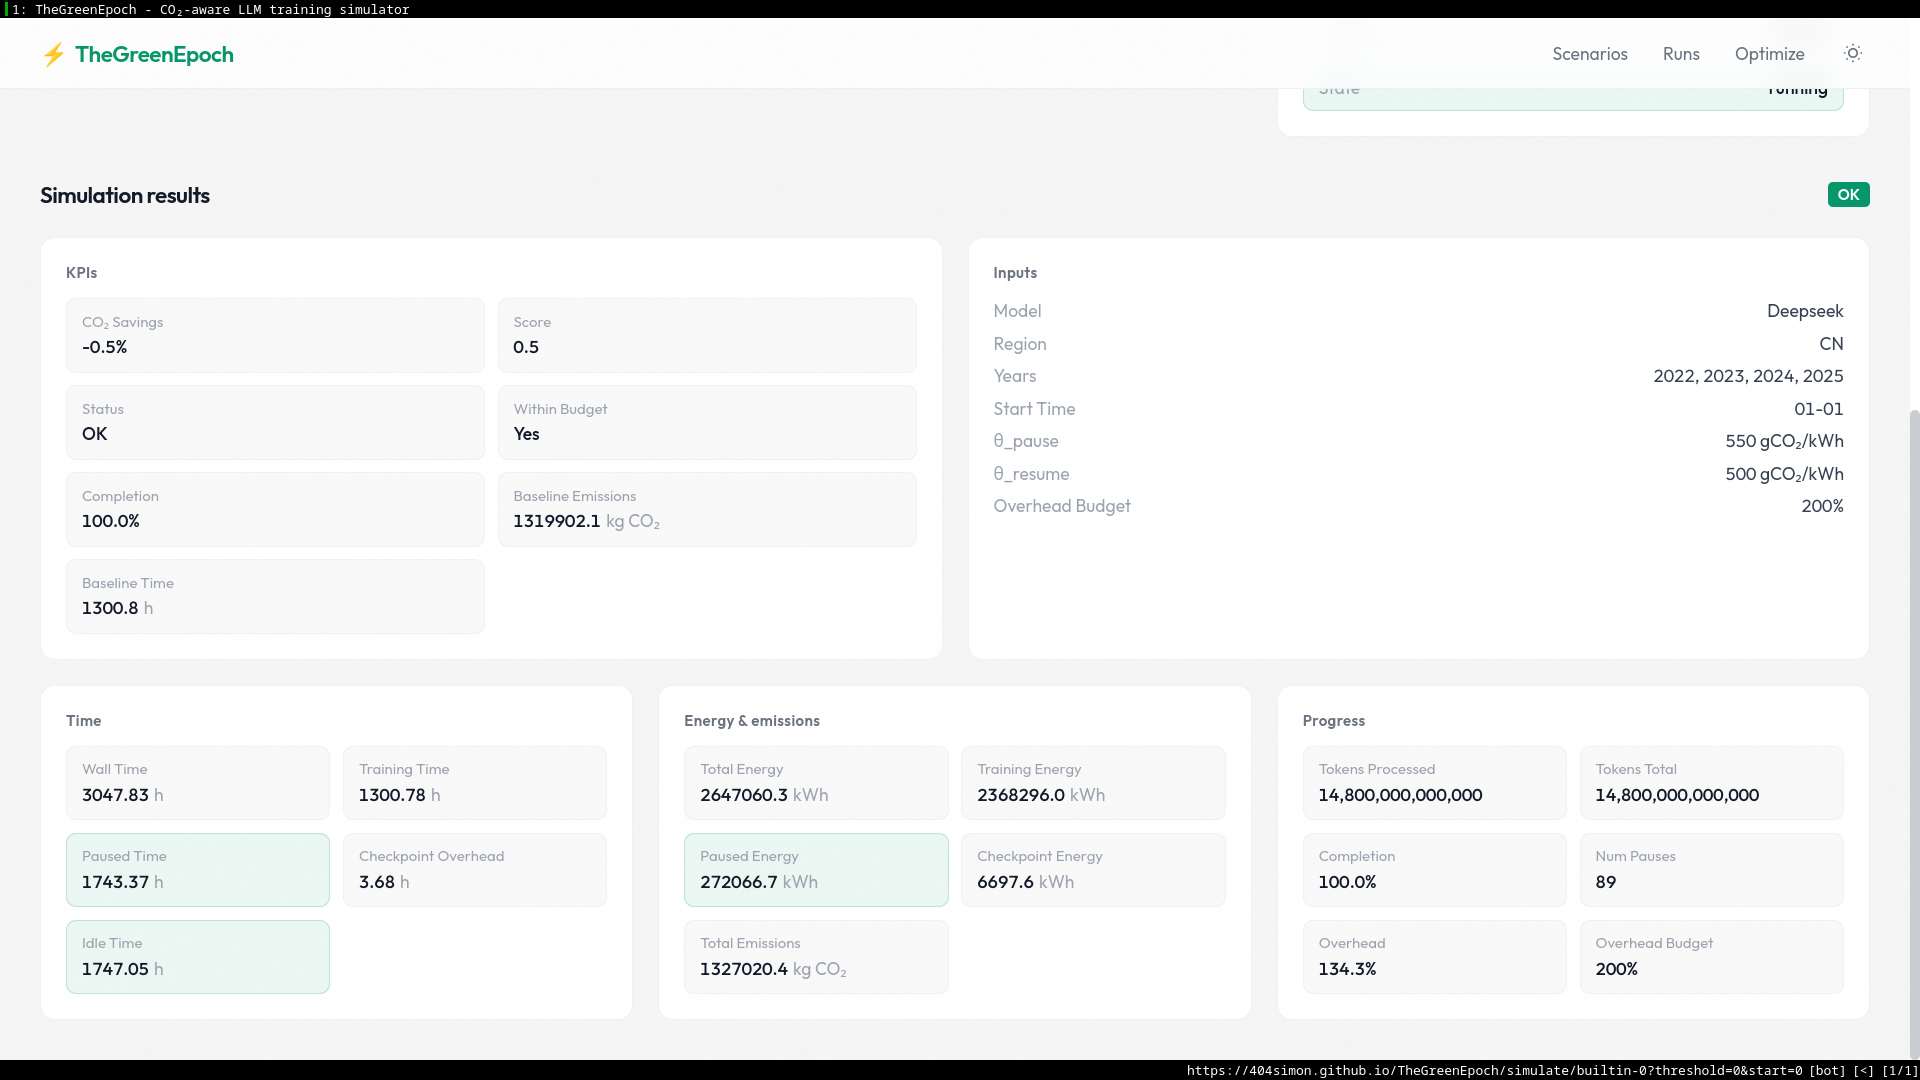
\includegraphics[width=\textwidth]{figures/screenshots/single_scenario_run_bottom_page}
  \caption{Single scenario run view (bottom): detailed KPIs comparing policy
  results against the never-pause baseline.}
  \label{fig:single-run-bottom}
\end{figure}

\section{Adaptive Optimizer}
\label{sec:optimizer-implementation}

The adaptive grid-search optimizer is implemented as a Web Worker that runs
iterations asynchronously.  Each iteration:
\begin{enumerate}
  \item Generates a grid of $(\theta_p, \theta_r, t_s)$ samples at the current
    resolution.
  \item Spawns individual simulation calls for each grid point.
  \item Collects results, scores them, and identifies the best point.
  \item Contracts the search bounds and reports progress to the UI.
\end{enumerate}

The optimizer posts \texttt{iteration} events after each zoom step, allowing
the UI to render intermediate results.  This gives the user real-time feedback
on convergence.

Figure~\ref{fig:optim-settings} shows the optimizer configuration panel where model, region, and algorithm parameters are selected. The resulting three-dimensional policy space is visualized in Figure~\ref{fig:optim-3d} as a color-coded scatter plot.

\begin{figure}
  \centering
  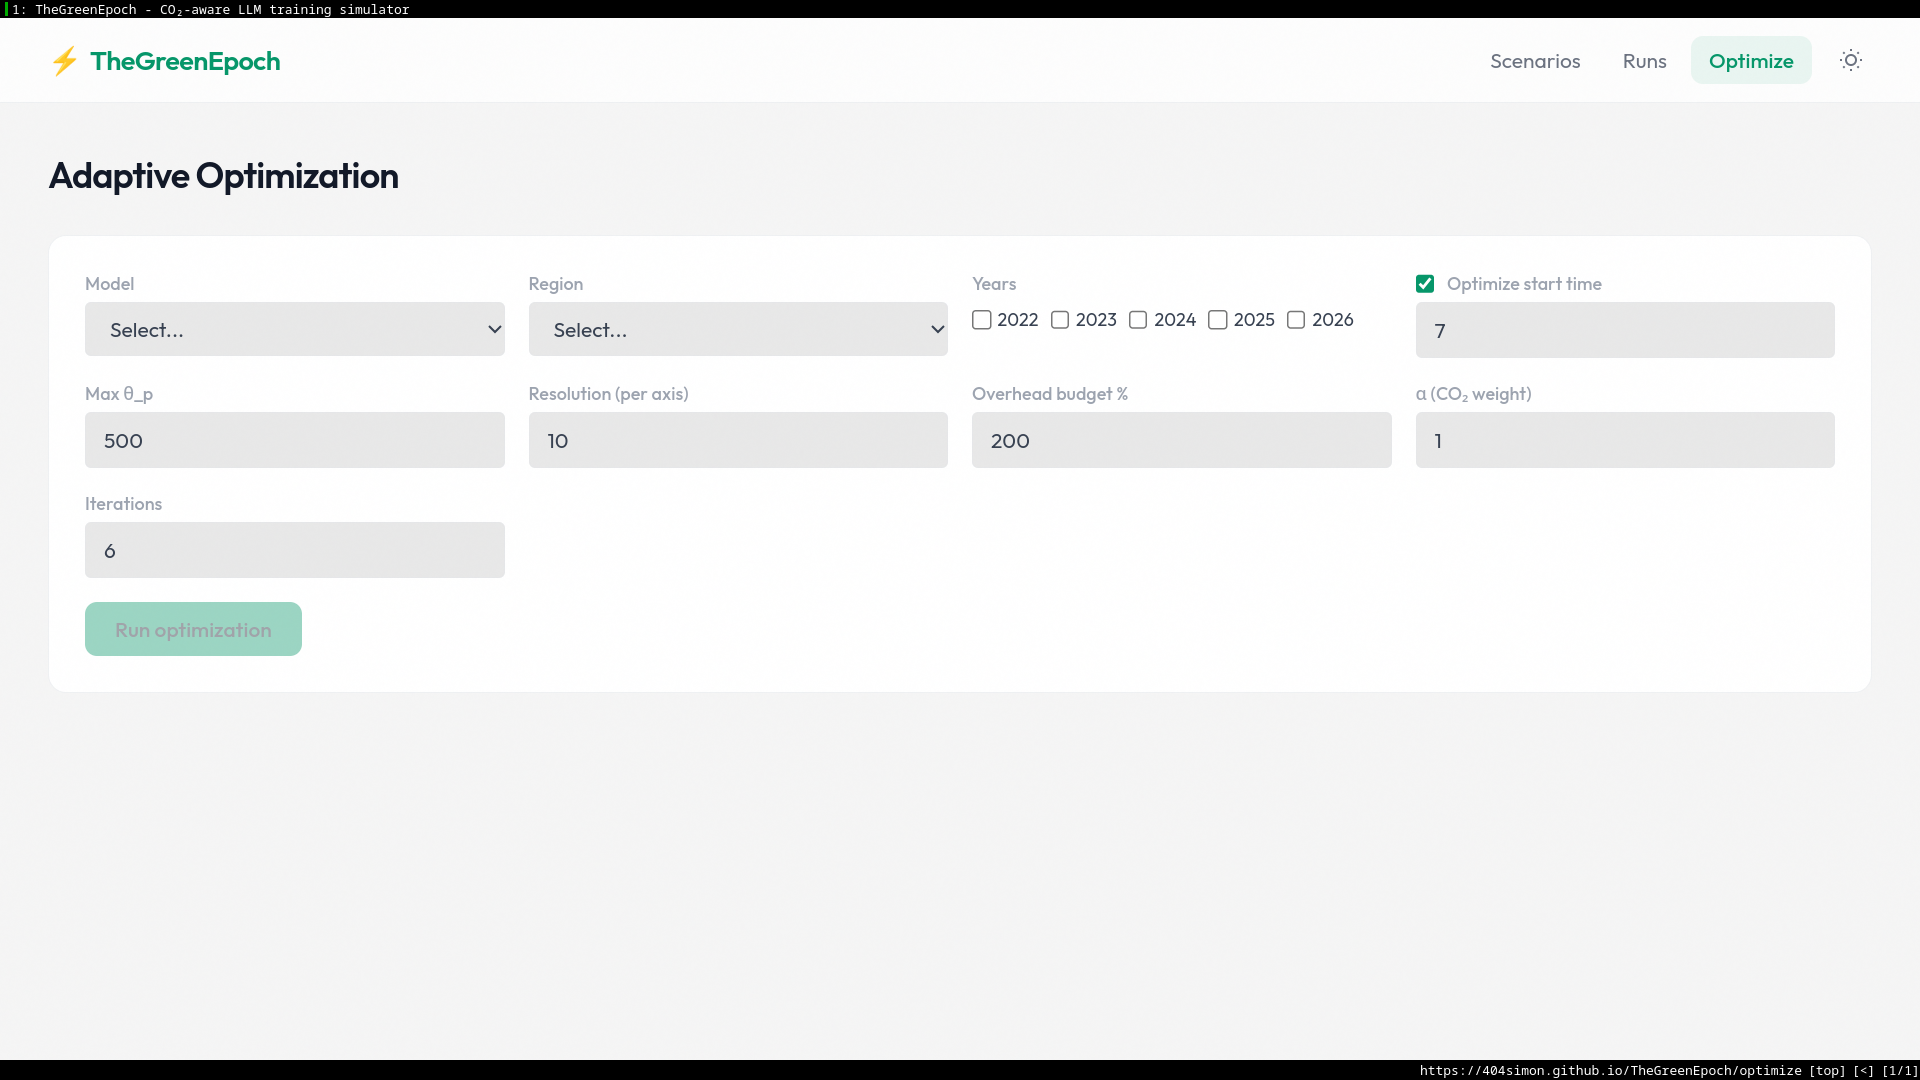
\includegraphics[width=\textwidth]{figures/screenshots/adaptive_optimization_page_settings}
  \caption{Optimization page settings panel: select model, region, years, and
  optimizer parameters.}
  \label{fig:optim-settings}
\end{figure}

\begin{figure}
  \centering
  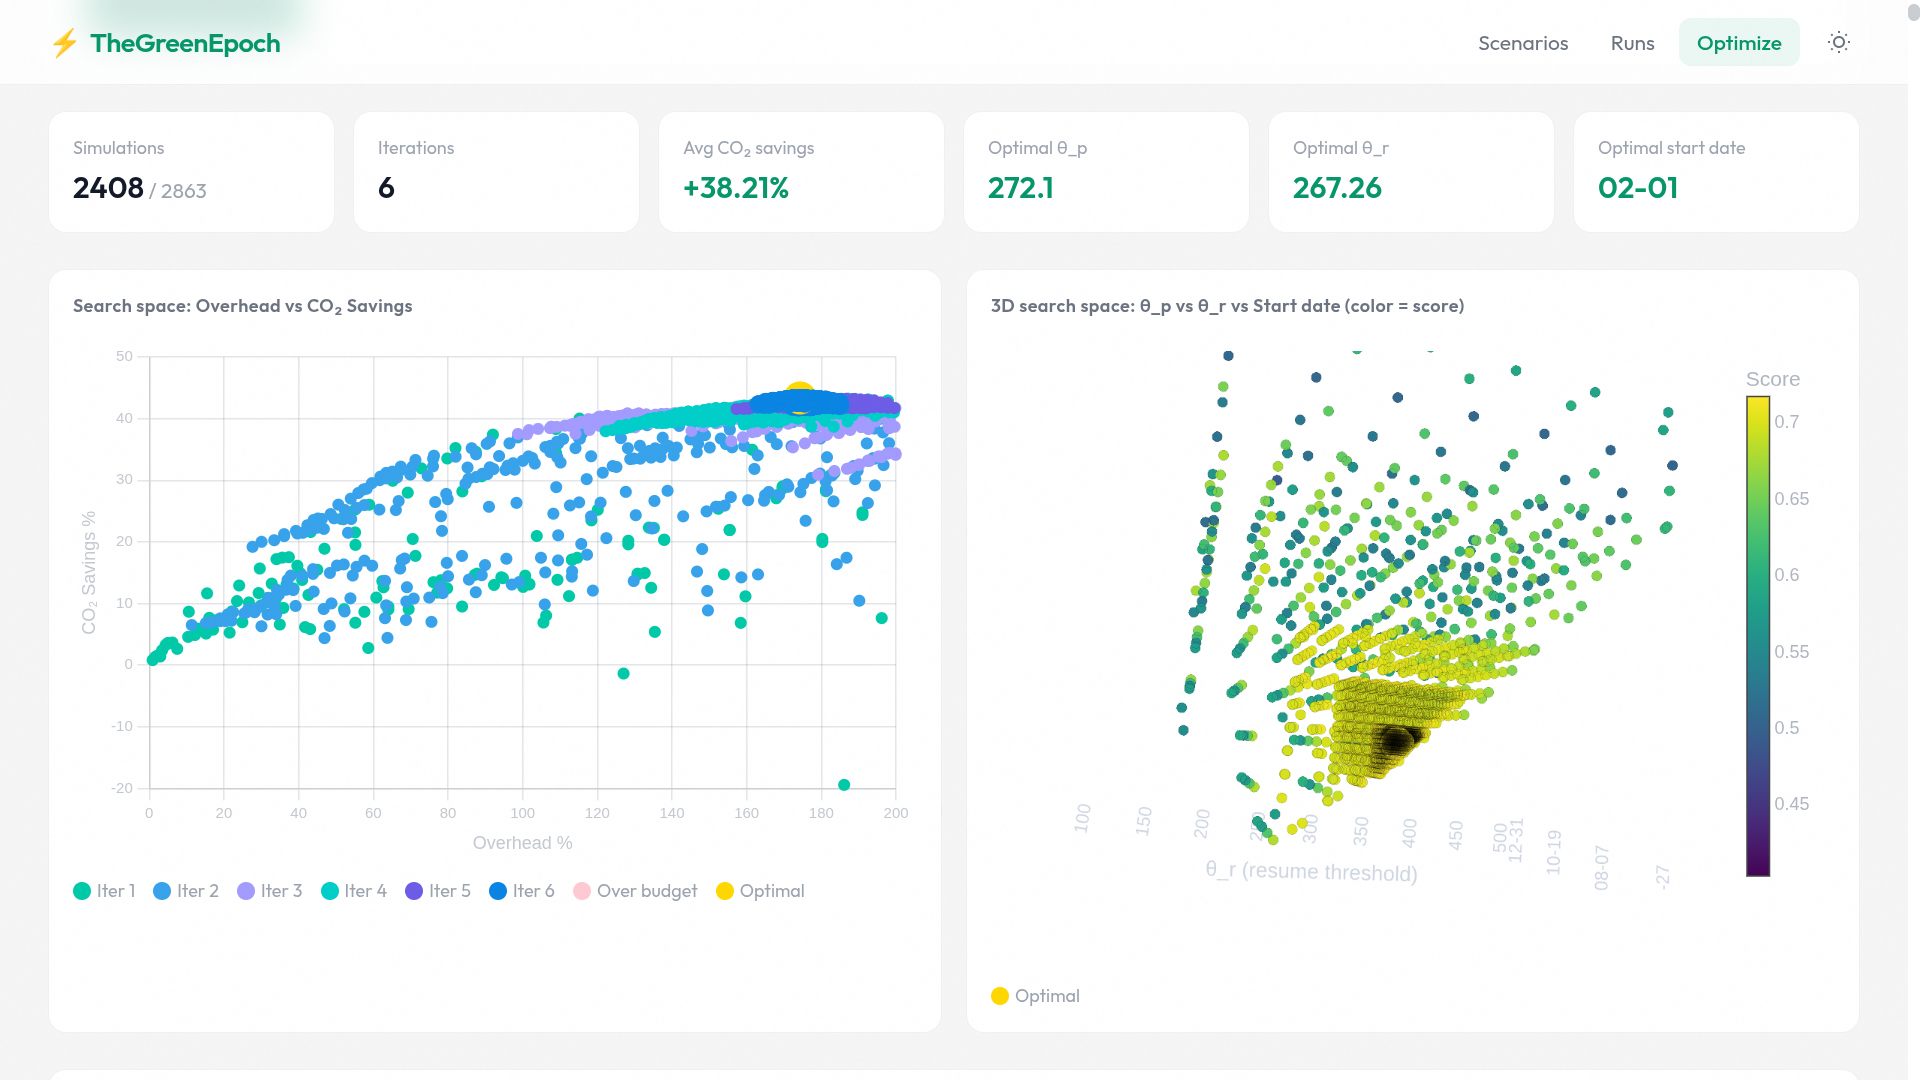
\includegraphics[width=\textwidth]{figures/screenshots/adaptive_optimization_page_results_middle_page_2}
  \caption{Optimization results: 3D scatter plot of pause threshold vs.\
  resume threshold vs.\ start date, colored by score.}
  \label{fig:optim-3d}
\end{figure}

\section{Batch Run Dashboard}
\label{sec:batch-dashboard}

The batch run page executes all configured scenarios across their threshold
and start-time combinations.  Results are displayed in a scatter plot
(overhead vs.\ CO$_2$ savings) and a sortable, filterable results table.  The
batch runner uses a dedicated Web Worker that processes scenarios sequentially
and posts results back progressively, providing a live progress indicator
(Figure~\ref{fig:batch-progress}). After completion, the scatter plot
(Figure~\ref{fig:batch-scatter}) visualizes the savings-overhead trade-off
across all evaluated configurations, and the sortable results table
(Figure~\ref{fig:batch-table}) provides detailed per-policy metrics.

\begin{figure}
  \centering
  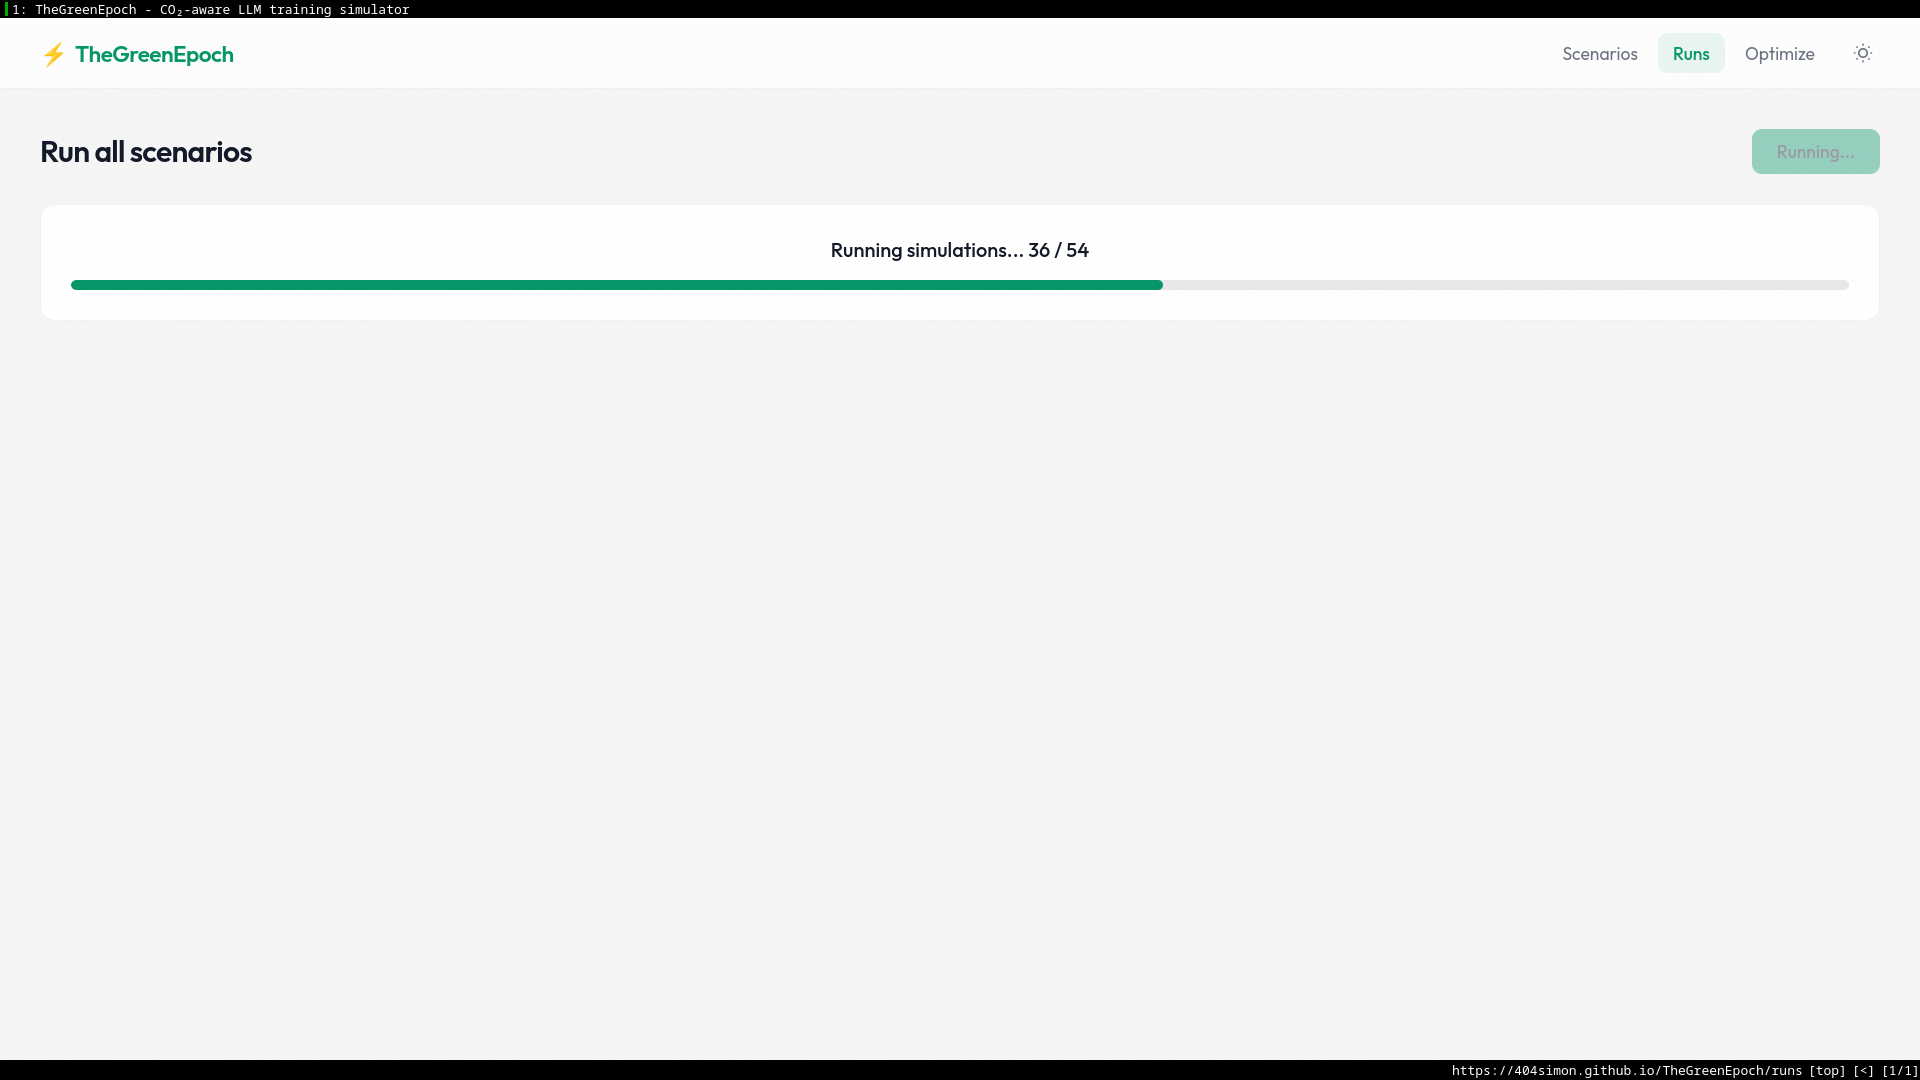
\includegraphics[width=\textwidth]{figures/screenshots/run_all_page_progress}
  \caption{Batch run dashboard showing progress and partial results during
  execution.}
  \label{fig:batch-progress}
\end{figure}

\begin{figure}
  \centering
  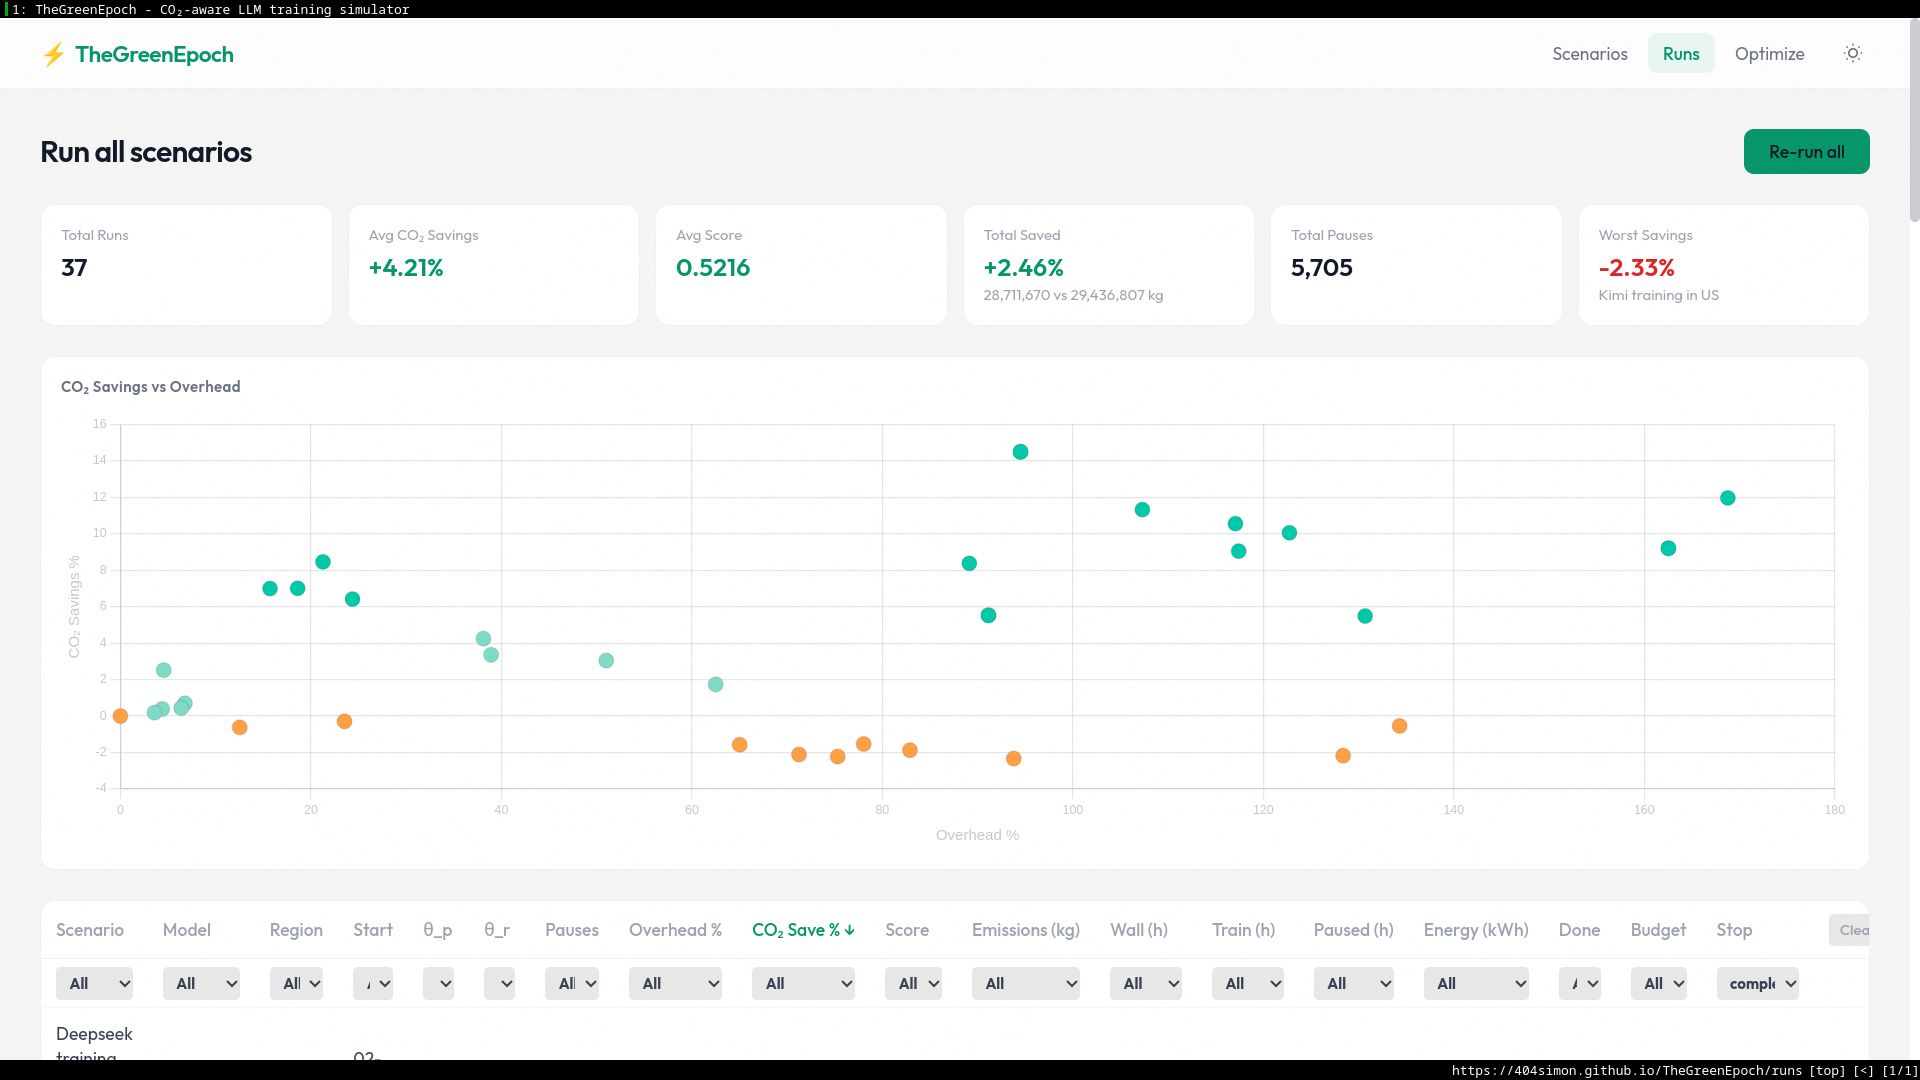
\includegraphics[width=\textwidth]{figures/screenshots/run_all_page_results_top_page}
  \caption{Batch run results view: scatter plot of CO$_2$ savings vs.\
  time overhead for all evaluated policies.}
  \label{fig:batch-scatter}
\end{figure}

\begin{figure}
  \centering
  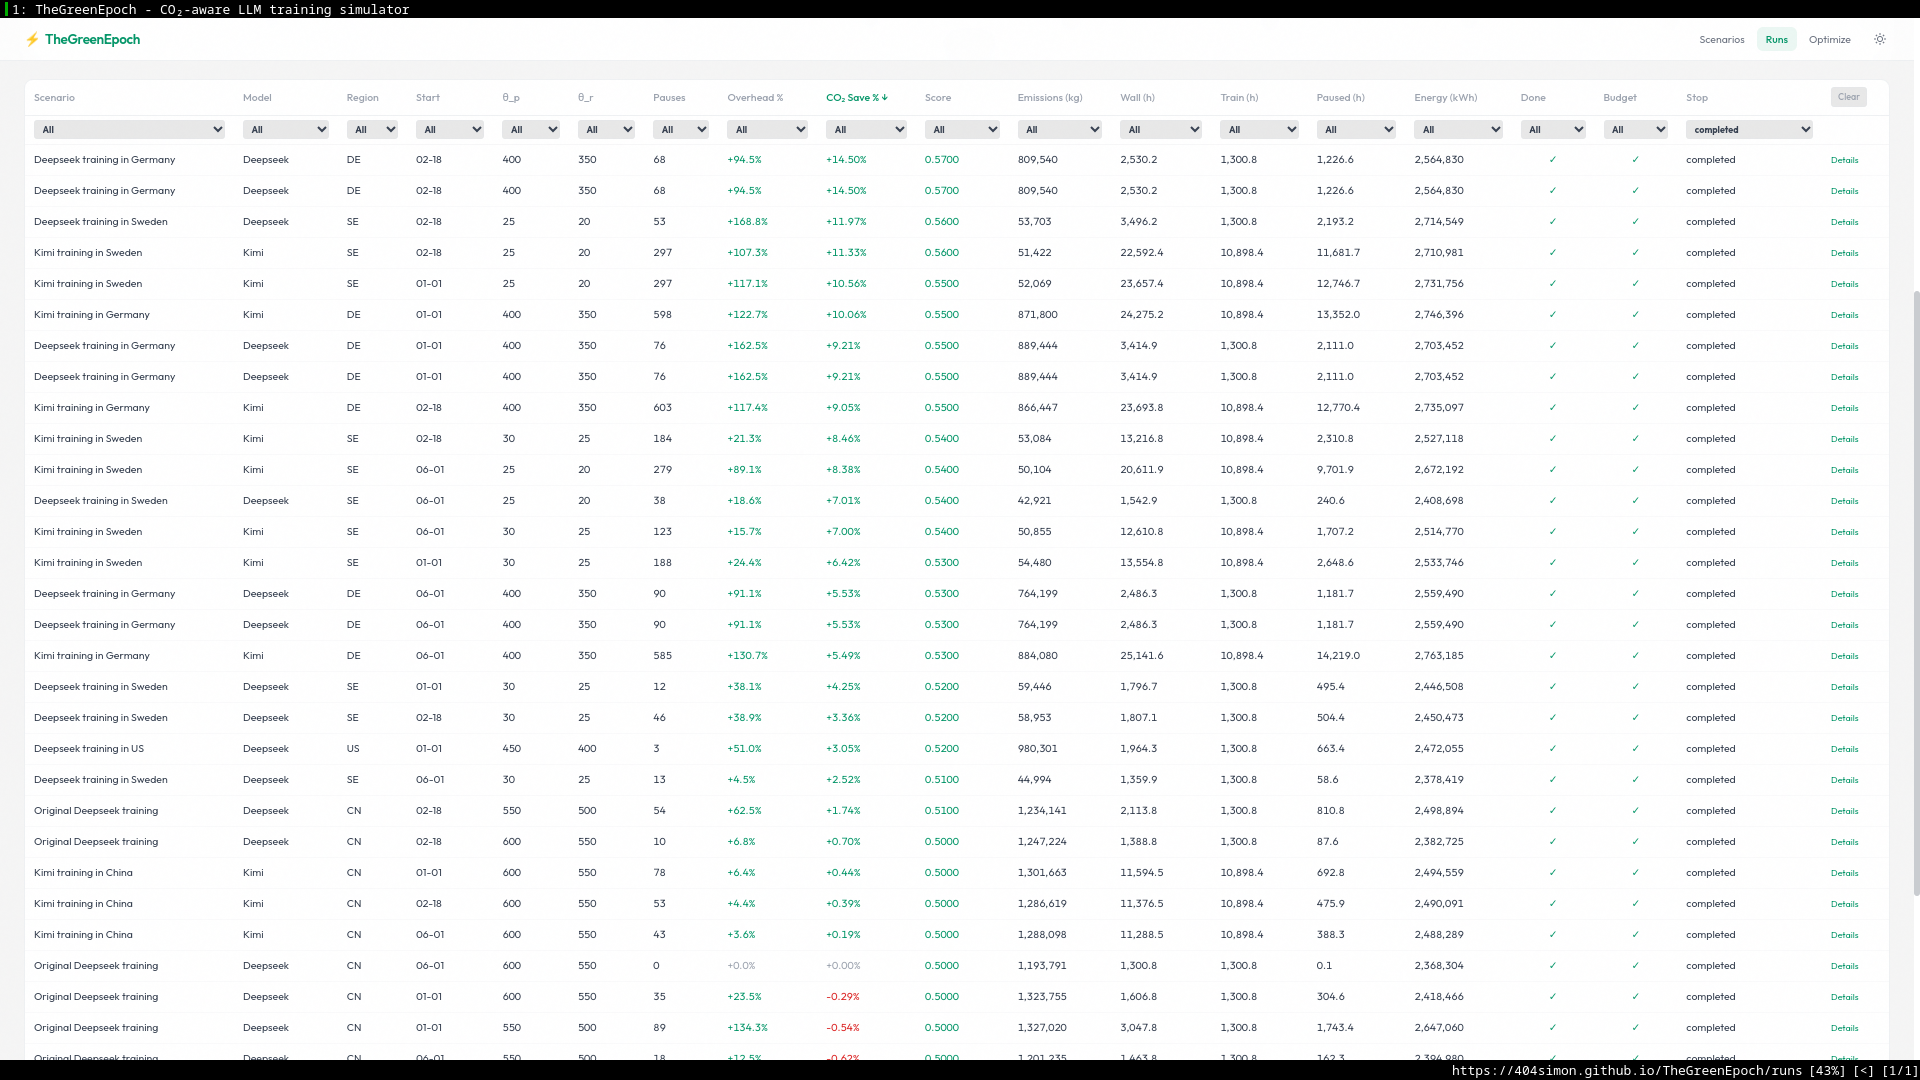
\includegraphics[width=\textwidth]{figures/screenshots/run_all_page_results_bottom_table}
  \caption{Batch run results table with sortable columns and detailed
  per-policy metrics.}
  \label{fig:batch-table}
\end{figure}

\section{Data Management}
\label{sec:data-management}

All data required for simulation is bundled with the application as static
JSON files:
\begin{itemize}
  \item \texttt{constants.json}: hardware constants (GPU power, power usage effectiveness,
    checkpoint overhead).
  \item \texttt{profiles.json}: training profiles for DeepSeek~V3 and
    Kimi~K2.
  \item \texttt{scenarios.json}: built-in default scenarios with preset
    parameters.
  \item \texttt{co2/*.json}: per-region, per-year CO$_2$ intensity time series
    at 5-minute resolution, pre-fetched from Electricity Maps.
\end{itemize}

User-created scenarios are persisted in the browser's localStorage.  The CO$_2$
data loader supports averaging multiple years into a representative timeline
and handles edge cases such as February 29 in leap years.

\section{CLI Tool}
\label{sec:cli}

In addition to the browser UI, the simulation and optimization engines are
exposed through a command-line interface using Commander.js.  The CLI supports
four commands:
\begin{itemize}
  \item \texttt{fetch}: download CO$_2$ intensity data from the Electricity
    Maps API for specified regions and date ranges.
  \item \texttt{run}: execute a batch of simulation scenarios and write
    results as CSV.
  \item \texttt{optimize}: run the adaptive grid-search optimizer from the
    command line and output the best policy configuration.
  \item \texttt{plot}: render optimization results as SVG charts for
    publication.
\end{itemize}

This dual-mode design (browser UI + CLI) ensures that the framework is useful
both for interactive exploration and for scripted, reproducible experiments.
